\documentclass[10pt]{article}



%Created on 4/10/07.

%\usepackage[OT1]{fontenc}
\usepackage{amsthm,amsmath,amssymb,bbm}
\usepackage{natbib}
\usepackage{multirow}
\usepackage[pdftex]{graphicx}
\usepackage{subfigure}
\usepackage{makecell}
\usepackage{booktabs}
\usepackage{array}
\usepackage{url}
\usepackage{algorithm}
\usepackage{algorithmic}
\usepackage{bm}
\usepackage{fullpage}
%\usepackage{mathtools}
\usepackage{wrapfig}
\usepackage{lipsum}
\usepackage{mathrsfs}
\usepackage{dsfont}
\usepackage{titling}
\usepackage{tikz}
%\usepackage{datetime}
%\usepackage{epstopdf,mathabx}

%\usepackage{algcompatible}
\usepackage{fancyhdr}
\pagestyle{fancy}
%\lhead{\today}
\rhead{ \today }
  \renewcommand{\footrulewidth}{0.4pt}% Line at the footer visible
\fancyfoot[C]{\thepage\ / \pageref{LastPage}}%

%\cfoot{center of the footer!}
%\renewcommand{\headrulewidth}{1pt}
%\renewcommand{\footrulewidth}{1pt}
\usepackage{multirow}
%\usepackage{subfigure}
%\usepackage{makecell}


%%%redefine the plain for first page
\usepackage{lastpage}
\fancypagestyle{plain}{%
  \fancyhf{}%
  \headsep=0.in
  \fancyhead[R]{\today}
 % \rhead{\thepage/\pageref{LastPage}}
  \fancyfoot[C]{\thepage\ / \pageref{LastPage}}%
  \renewcommand{\headrulewidth}{0.4pt}% Line at the header invisible
  \renewcommand{\footrulewidth}{0.4pt}% Line at the footer visible
}
%%%%%

\def\skeptic{{\sc skeptic}}
\newcommand{\sgn}{\mathop{\mathrm{sign}}}
\providecommand{\norm}[1]{\|#1\|}
\providecommand{\bnorm}[1]{\big\|#1\big\|}
\providecommand{\enorm}[1]{| \! | \! |#1| \! | \! |}
\providecommand{\bemnorm}[1]{\big| \! \big| \! \big|#1\big| \! \big| \! \big|}


%%%%My macros 
\usepackage{slada}
\newcommand*{\Sc}{\cS^{\perp}}
\newcommand*{\Ac}{\cA^{\perp}}
\newcommand*{\supp}{\mathrm{supp}}
%\usepackage{cite}
\newcommand \rw{\mathrm{w}}
\newcommand{\nn}{\nonumber}

\newcommand{\E}{\mathbb{E}}
\newcommand{\pp}{\mathbb{P}}
\newcommand{\reals}{\mathbb{R}}
\newcommand{\nats}{\mathbb{N}}
\newcommand{\var}{\text{Var}}
\newcommand{\indepdist}{\overset{\text{ind.}}{\sim}}

%%%%Definition of Operators
\newcommand {\vecc}{\textnormal {vec}}
\def\T{\mathrm{\scriptstyle T}} %%%transpose operator
\def\sn{\sum_{i=1}^n}
\newcommand {\summ}{\textnormal {sum}}


%%%%Definition of Roman Numbers
\newcommand{\Rom}[1]{\text{\uppercase\expandafter{\romannumeral #1\relax}}}




%%%%Definition of Equation environment
\def\##1\#{\begin{align}#1\end{align}}
\def\$#1\${\begin{align*}#1\end{align*}}


\usetikzlibrary{shapes,decorations,arrows,calc,arrows.meta,fit,positioning}
\tikzset{
    -Latex,auto,node distance =1 cm and 1 cm,semithick,
    state/.style ={ellipse, draw, minimum width = 0.7 cm},
    point/.style = {circle, draw, inner sep=0.04cm,fill,node contents={}},
    bidirected/.style={Latex-Latex,dashed},
    el/.style = {inner sep=2pt, align=left, sloped}
}

\newcommand{\indep}{\rotatebox[origin=c]{90}{$\models$}}

%head separation
\setlength{\headsep}{0.2in}
 

\renewcommand{\baselinestretch}{1.1}

\usepackage{enumitem}
\begin{document}

\title{\LARGE \bf Notes for "Hernán MA, Robins JM (2019). Causal Inference. Boca Raton: Chapman and Hall/CRC, forthcoming."} 
\author{Alex Gao }
\date{}

\maketitle
\vspace{-0.6in}

These notes are for personal understanding and they most certainly will have typos and errors as they develop. Please read with care.

\section{Chapter 1 - 3}

\textbf{Definition (Consistency):} This is the assumption that $Y = Y^A$, where Y is the response and A is the binary treatment. The implications of this are: $\E (Y^{a=1} | A = 1) = \E (Y | A = 1)$ and likewise for $A = 0$.\\

Consider the following causal DAG:\\

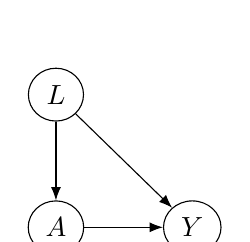
\begin{tikzpicture}
    \node[state] (a) at (0,0) {$A$};
    \node[state] (y) [right=of a] {$Y$};
    \node [state] (l) [above=of a] {$L$};

    \path (a) edge (y);
    \path (l) edge (a);
    \path (l) edge (y);

\end{tikzpicture}

L are covariates, A is the binary treatment, Y is the binary response. Suppose that a randomized control trial is performed. Then the resulting DAG will look like this:\\

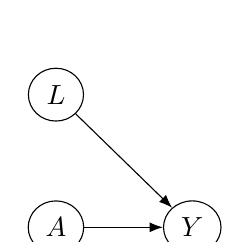
\begin{tikzpicture}
    \node[state] (a) at (0,0) {$A$};
    \node[state] (y) [right=of a] {$Y$};
    \node [state] (l) [above=of a] {$L$};

    \path (a) edge (y);
    \path (l) edge (y);

\end{tikzpicture}\\

\noindent \textbf{Definition (Full Exchangeability):} $(Y^{a=0}, Y^{a=1}) \indep A$
	
\noindent \textbf{Definition (Exchangeability):} $Y^a \indep A, \forall a$

\noindent \textbf{Definition (Mean Exchangeability):} $\E (Y^a | A = 1) = \E(Y^a | A = 0), \forall a$\\

Note that full exchangeability $\implies$ exchangeability $\implies$ mean exchangeability. \\

\noindent \textbf{Remark:} Randomized control trials produce exchangeability implying that association is equivalent to causation. To see this: By consistency assumption, we have $\pp (Y = 1 | A = 1) = \pp(Y^{a=1} = 1 | A = 1)$. Furthermore, by randomization we have exchangeability so $\pp(Y^{a=1} = 1 | A = 1) = \pp(Y^{a=1} = 1)$. Hence we have $\pp (Y = 1 | A = 1) = \pp(Y^{a=1} = 1)$, where the LHS can we estimated with the observed data. Likewise, a similar argument can be used to show that $\pp (Y = 1 | A = 0) = \pp(Y^{a=0} = 1)$.

\subsection{Inverse probability weighting estimators}

Define $f(a | l)$ to be the conditional probability distribution of $A | L$. Then:

\begin{equation}
\begin{aligned}
\EE \left( \frac{ I(A=a) Y}{ f(A|L) } \right)  &= \EE \left( \EE \left( \frac{ I(A=a) Y}{ f(A|L) } | A,L \right) \right) \\
&= \sum_l \sum_{a'} \EE \left( \frac{ I(A=a) Y}{ f(a'|l) } | A = a', L = l \right) \pp (A = a' | L = l) \pp(L = l) \\
&= \sum_l \sum_{a'} \EE \left( \frac{ I(A=a) Y}{ f(a'|l) } | A = a', L = l \right) f(a' | l) \pp(L = l), \text{ by definition} \\
&= \sum_l \EE(Y| A=a, L = l' ) \pp(L = l') \\
&= \EE(Y^{A=a}), \text{ by the adjustment formula }
\end{aligned}
\end{equation}



\end{document}






